\chapter[cakirxVya saMKeyxgaLu ({\rm\bfseries Cyclic Numbers})]{cakirxVya saMKeyxgaLu\\ ({\rm\bfseries Cyclic Numbers})}
\vskip -20pt

$2,3$ matutx $5$ nunx biTuTx ELu eMba aviBAjayx saMKeyxyiMda oMdanunx BAgisidAga, BAgalabadhxdalilx baruva oMdu guMpu aMkagaLu punarAvatiRsutatxve. ivugaLanunx AvataRka dashamAMsha aMkagaLu enunxtetxVve.
$$
\frac{1}{7} = 0.14285{\dot 7}
$$
ililx eDatudiyalilxruva dashamAMsha biMdu matutx balatudiya koneya aMkada meVliruva AvataRsUcaka biMduvanunx biTuTx biTaTxre. $142857$ barutatxde. idoMdu {\bf cakirxVya saMKeyx} EkeMdare $7$ kikxMta kaDime pUNARMkagaLiMda guNisidare baruva guNalabadhxdalilx saMKeyxgaLu cakirxVyavAgirutatxve.

\begin{tabular}[c]{>{$}l<{$}}
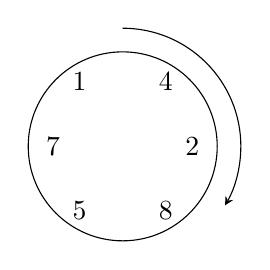
\begin{tikzpicture}[label distance=0.5cm]%%m_073
\draw (1,1) node[circle,
label=60:$4$,label=120:$1$,label=180:$7$, label=240:$5$,
label=300:$8$, label=360:$2$]{}circle(1.2cm);
\draw [>=stealth,->] (1,2.5) arc [radius=1.5, start angle=90, end angle= -30];
\end{tikzpicture}
\end{tabular}
\hspace{0.5cm}
\begin{tabular}[c]{>{$}l<{$}>{$}l<{$}}
142857 \times 1 &= 142857\\
142857 \times 2 &= 285714\\
142857 \times 3 &= 428571\\
142857 \times 4 &= 571428\\
142857 \times 5 &= 714285\\
142857 \times 6 &= 857142
\end{tabular}

I saMKeyxgaLalilx $3,6,0$ matutx $9$ elUlx baMdilalx.

ideV riVti $17$ riMda $1$ nunx BAgisidare
\begin{align*}
\frac{1}{17} &= 0.0588235294117647\\
&\qquad 0588235294117647 \quad\text{oMdu cakirxVya saMKeyx}
\end{align*}
\begin{align*}
0588235294117647 \times 1 &= 0588235294117647\\
~~~~~~\shortparallel ~~~~~~~~~~~~~ \times 2 &= \\
~~~~~~\shortparallel ~~~~~~~~~~~~~\times 3 &= \\
~~~~~~\shortparallel ~~~~~~~~~~~~~\times 4 &= \\
~~~~~~\shortparallel ~~~~~~~~~~~~~\times 5 &= \\
~~~~~~\shortparallel ~~~~~~~~~~~~~\times 6 &= \\
~~~~~~\shortparallel ~~~~~~~~~~~~~\times 7 &= \\
~~~~~~\shortparallel ~~~~~~~~~~~~~\times 8 &= \\
~~~~~~\shortparallel ~~~~~~~~~~~~~\times 9 &= \\
~~~~~~\shortparallel ~~~~~~~~~~~\times 10 &= \\
~~~~~~\shortparallel ~~~~~~~~~~~\times 11 &= \\
~~~~~~\shortparallel ~~~~~~~~~~~\times  12&= \\
~~~~~~\shortparallel ~~~~~~~~~~~\times  13&= \\
~~~~~~\shortparallel ~~~~~~~~~~~\times  14&= \\
~~~~~~\shortparallel ~~~~~~~~~~~\times  15&= \\
~~~~~~\shortparallel ~~~~~~~~~~~\times  16&= 
\end{align*}
oMdariMda hadinArara tanaka saMKeyxgaLiMda guNisidAga guNalabadhx cakirxVyavAgirutatxde.

ideV riVti $1$ nunx $13$ riMda BAgisidAga baruva $076923$ iMdu cakirxVya saMKeyx
$$
\frac{1}{13} = 0.076923
$$
\begin{align*}
076923 \times 1 &= 076923 \\
~~~~~~~~~\shortparallel ~~~\times 3 &= 230769 \\ 
~~~~~~~~~\shortparallel ~~~\times 4 &= 923076 \\
~~~~~~~~~\shortparallel ~~~\times 9 &= 692307 \\ 
~~~~~~~~~~~\shortparallel ~\times 10 &= 769230 \\
076923\times 12 &= 923076\\[5pt] 
076923 \times 2 &= 153846 \\
~~~~~~~~~\shortparallel ~~~\times 5 &= 384615 \\
076923   \times 6 &= 461538 \\
~~~~~~~~~\shortparallel ~~~\times 7 &= 538461 \\
~~~~~~~~~\shortparallel ~~~\times 8 &= 615384 \\
~~~~~~~~~~~\shortparallel ~\times 11 &= 846153 
\end{align*}

$076923$ nunx  I eraDu riVtiya saMKeyxgaLiMda guNisidare mAtarx saMKeyxgaLu cakirxVyavAgi barutatxve. modalaneya guMpinalilxruva saMKeyxgaLu eraDaneya guMpinalilxlalx. aMtU saMKeyxgaLa vinAyxsaveV oMdu sobagu.
